%!TEX root =presentation.tex
\section{Ramp metering} % (fold)
\label{sec:demo_ramp_metering}

% section demo_ramp_metering (end)

\begin{frame}{Discrete adjoint method applied to ramp metering}

\begin{figure}
\begin{centering}
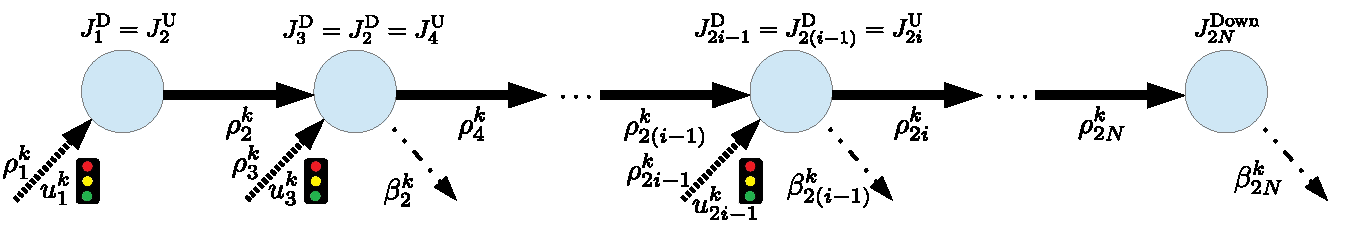
\includegraphics[width=1\columnwidth]{../figs-gen/rm-junction-2}
\par\end{centering}
\end{figure}

\begin{itemize}
\item For a junction $\jdown{2\link-1}=\jdown{2\left(\link-1\right)}=\jup{2\link}$ at time-step $\tind\in\intrange 0{\ntime-1}$.
\item Upstream mainline density: $\densitydiscrete{2\left(\link-1\right)}{\tind}$.
 \item Downstream mainline density: $\densitydiscrete{2\link}{\tind}$.
 \item Onramp density: $\densitydiscrete{2\link-1}{\tind}$
 \item Offramp split ratio: $\splitratio_{2\left(\link-1\right)}^{\tind}$.
\end{itemize}


\end{frame}

\begin{frame}{Governing Equations}
\begin{block}{Mainline equations}
\begin{eqnarray*}
\syseq_{2\link}^{\tind}(\state,\control)= & \discrete{2\link}{\tind}-\discrete{2\link}{\tind-1} & +\frac{\Delta t}{\length_{2\link}}\left(\fout{2\link}{\tind-1}-\fin{2\link}{\tind-1}\right)=0
	\end{eqnarray*}
\end{block}

\begin{block}{Onramp equations}
\begin{eqnarray*}
\syseq_{2\link-1}^{\tind}(\state,\control) & = & \discrete{2\link-1}{\tind}-\discrete{2\link-1}{\tind-1}+\frac{\Delta t}{\length_{2\link-1}}\left(\fout{2\link-1}{\tind-1}-\boundaryDemand{2\link-1}{\tind-1}\right)=0
 \end{eqnarray*}
\end{block}

\end{frame}

\begin{frame}{Flux solutions}
\begin{eqnarray}
\demand_{2\left(\link-1\right)}^{\tind} & = & \min\left(\ffspeed_{2\left(i-1\right)}\densitydiscrete{2\left(\link-1\right)}{\tind},F_{2\left(\link-1\right)}^{\max}\right)\label{eq:first-ramp}\\
\supply_{2\link}^{\tind} & = & \min\left(\congspeed_{2i}\left(\density_{2i}^{\max}-\densitydiscrete{2\link}{\tind}\right),F_{2i}^{\max}\right)\label{eq:supply}\\
\rampDemand_{2\link-1}^{\tind} & = & \ramp_{2\link-1}^{\tind}\min\left(\frac{\length_{2\link-1}}{\Delta t}\densitydiscrete{2\link-1}{\tind},F_{2i-1}^{\max}\right)\label{eq:ramp-eqn}\\
\fin{2\link}{\tind} & = & \min\left(\splitratio_{2\left(\link-1\right)}^{\tind}\demand_{2\left(\link-1\right)}^{\tind}+\rampDemand_{2\link-1}^{\tind},\supply_{2\link}^{\tind}\right)\label{eq:fin}
\end{eqnarray}

\begin{figure}
\begin{centering}
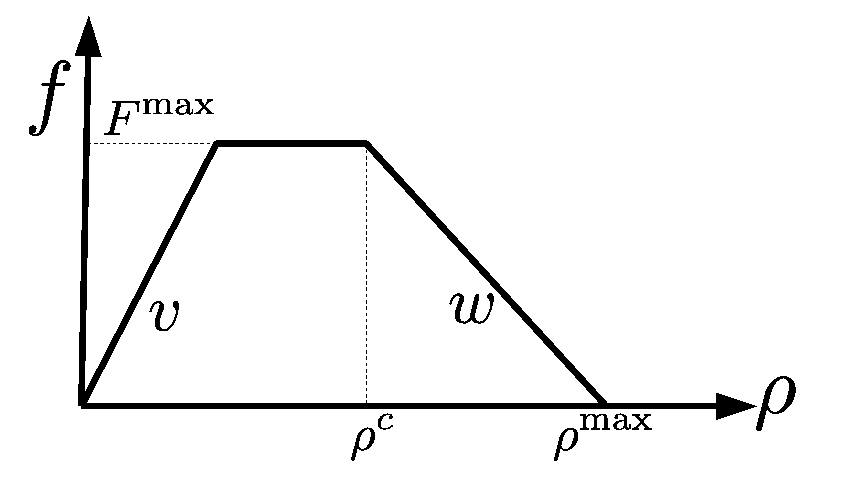
\includegraphics[width=0.4\columnwidth]{../figs-gen/fd}
\par\end{centering}
\end{figure}

\end{frame}


\begin{frame}{Flux solutions}
\begin{eqnarray}
\demand_{2\left(\link-1\right)}^{\tind} & = & \min\left(\ffspeed_{2\left(i-1\right)}\densitydiscrete{2\left(\link-1\right)}{\tind},F_{2\left(\link-1\right)}^{\max}\right)\label{eq:first-ramp}\\
\supply_{2\link}^{\tind} & = & \min\left(\congspeed_{2i}\left(\density_{2i}^{\max}-\densitydiscrete{2\link}{\tind}\right),F_{2i}^{\max}\right)\label{eq:supply}\\
\rampDemand_{2\link-1}^{\tind} & = & \ramp_{2\link-1}^{\tind}\min\left(\frac{\length_{2\link-1}}{\Delta t}\densitydiscrete{2\link-1}{\tind},F_{2i-1}^{\max}\right)\label{eq:ramp-eqn}\\
\fin{2\link}{\tind} & = & \min\left(\splitratio_{2\left(\link-1\right)}^{\tind}\demand_{2\left(\link-1\right)}^{\tind}+\rampDemand_{2\link-1}^{\tind},\supply_{2\link}^{\tind}\right)\label{eq:fin}\\
\fout{2\left(\link-1\right)}{\tind} & = & \begin{cases}
\demand_{2\left(\link-1\right)}^{\tind} & \frac{p_{2(\link-1)}\fin{2\link}{\tind}}{\splitratio_{2\left(\link-1\right)}^{\tind}\left(1+p_{2(\link-1)}\right)}\ge\demand_{2\left(\link-1\right)}^{\tind}\hfill\text{[C1]}\\
\frac{\fin{2\link}{\tind}-\rampDemand_{2\link-1}^{\tind}}{\splitratio_{2\left(\link-1\right)}^{\tind}} & \frac{\fin{2\link}{\tind}}{1+p_{2(\link-1)}}\ge\rampDemand_{2\link-1}^{\tind}\hfill\text{[C2]}\\
\frac{p_{2(\link-1)}\fin{2\link}{\tind}}{\left(1+p_{2(\link-1)}\right)\splitratio_{2\left(\link-1\right)}^{\tind}} & \text{otherwise}\hfill\text{[C3]}
\end{cases}\label{eq:merge}\\
\fout{2\link-1}{\tind} & = & \fin{2\link}{\tind}-\splitratio_{2\left(\link-1\right)}^{\tind}\fout{2\left(\link-1\right)}{\tind}\label{eq:last-ramp}
\end{eqnarray}
\end{frame}

\begin{frame}{Partial derivates for adjoint method}
\fontsize{6pt}{7.2}\selectfont
\begin{eqnarray*}
\pfrac{\demand_{2\left(\link-1\right)}^{\tind}}s & = & \begin{cases}
\ffspeed_{2\left(i-1\right)} & s=\densitydiscrete{2\left(\link-1\right)}{\tind},\ffspeed_{i}\densitydiscrete{2\left(\link-1\right)}{\tind}\le F_{2\left(i-1\right)}^{\max}\\
0 & \text{otherwise}
\end{cases}\\
\pfrac{\supply_{2\link}^{\tind}}s & = & \begin{cases}
-\congspeed_{2i} & s=\densitydiscrete{2\link}{\tind},\congspeed_{2i}\left(\density_{2i}^{\max}-\densitydiscrete{2\link}{\tind}\right)\le F_{2i}^{\max}\\
0 & \text{otherwise}
\end{cases}\\
\pfrac ds & = & \begin{cases}
\ramp_{2\link-1}^{\tind} & s=\densitydiscrete{2\link-1}{\tind},\densitydiscrete{2\link-1}{\tind}\le F_{2\link-1}^{\max}\\
\min\left(\densitydiscrete{2\link-1}{\tind},F_{2i-1}^{\max}\right) & s=\ramp_{2\link-1}^{\tind}\\
0 & \text{otherwise}
\end{cases}\\
\pfrac{}s\fin{2\link}{\tind} & = & \begin{cases}
\splitratio_{2\left(\link-1\right)}^{\tind}\pfrac{\demand_{2\left(\link-1\right)}^{\tind}}s+\pfrac{\rampDemand_{2\left(\link-1\right)}^{\tind}}s & \splitratio_{2\left(\link-1\right)}^{\tind}\demand_{2\left(\link-1\right)}^{\tind}+\rampDemand_{2\link-1}^{\tind}\le\supply_{2\link}^{\tind}\\
\pfrac{\supply_{2\link}^{\tind}}s & \text{otherwise}
\end{cases}\\
\pfrac{}s\fout{2\left(\link-1\right)}{} & = & \begin{cases}
\pfrac{\demand_{2\left(\link-1\right)}^{\tind}}s & \frac{\fin{2\link}{\tind}p_{2(\link-1)}}{1+p_{2(\link-1)}}\ge\frac{\demand_{2\left(\link-1\right)}^{\tind}}{\splitratio_{2\left(\link-1\right)}^{\tind}}\\
\frac{1}{\splitratio_{2\left(\link-1\right)}^{\tind}}\left(\pfrac{}s\fin{2\link}{\tind}-\pfrac{\rampDemand_{2\link-1}^{\tind}}s\right) & \frac{\fin{2\link}{\tind}}{1+p_{2(\link-1)}}\ge\rampDemand_{2\left(\link-1\right)}^{\tind}\\
\frac{p_{2(\link-1)}}{\splitratio_{2\left(\link-1\right)}^{\tind}\left(1+p_{2(\link-1)}\right)}\pfrac{}s\fin{2\link}{\tind} & \text{otherwise}
\end{cases}\\
\pfrac{}s\fout{2\link-1}{} & = & \pfrac{}s\fin{2\link}{\tind}-\splitratio_{2\left(\link-1\right)}^{\tind}\pfrac{}s\fout{2\left(\link-1\right)}{}
\end{eqnarray*}
\end{frame}

\begin{frame}{Numerical results}

\begin{block}{Network}
\begin{itemize}
\item I15 South in San Diego, CA, USA.
\item 19.4 miles.
\item 125 discrete links.
\item 9 onramps.
\item Scaled flow data from real loop detector data.
\end{itemize}

\begin{figure}
\begin{centering}
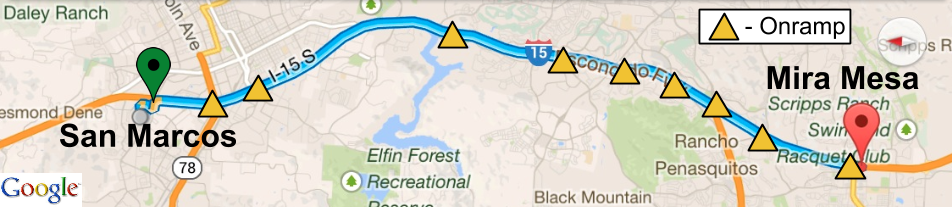
\includegraphics[width=0.6\columnwidth]{../images/map}
\par\end{centering}
\end{figure}

\end{block}

\end{frame}

\begin{frame}{Numerical results}

\begin{block}{Comparative methods}
\begin{itemize}
	\item Adjoint method
	\item *Finite differences (No gradient information).
	\item Alinea [1]
	\item No control
\end{itemize}
*Finite differences becomes impractical for even very small networks.

\begin{figure}
\begin{centering}
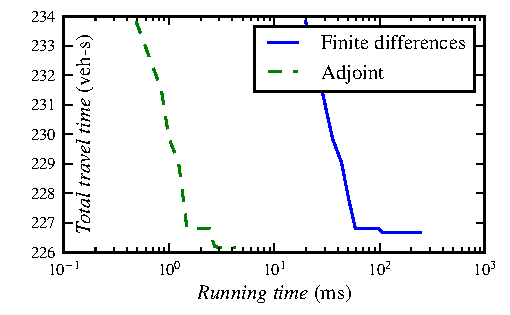
\includegraphics[width=0.4\columnwidth]{../images/itergrad}
\par\end{centering}
\end{figure}
\end{block}

[1] Papageorgiou et al

\end{frame}

\begin{frame}{Open loop optimal control}

\begin{figure}
\subfloat[Density difference profile in units of vehicles per mile.\label{fig:long-sim-density}]{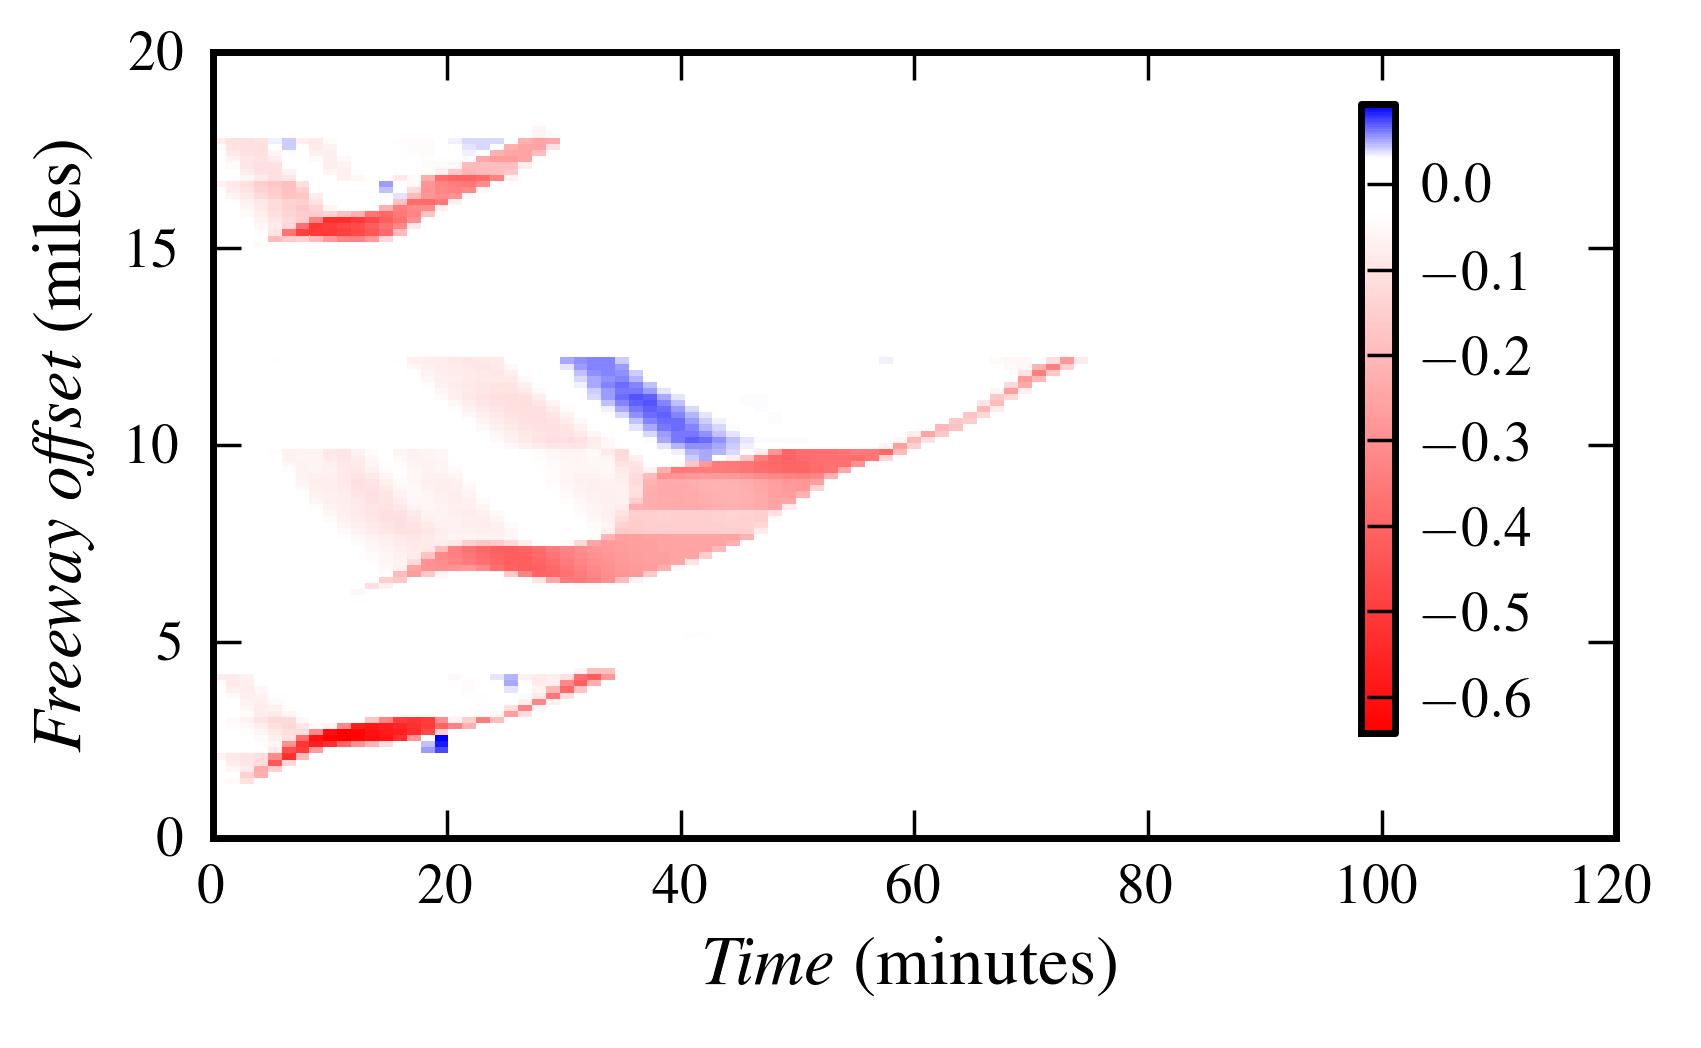
\includegraphics[width=0.45\columnwidth]{../images/densdiff}

}\hfill{}\subfloat[Queue difference profile in units of vehicles.\label{fig:long-sim-queue}]{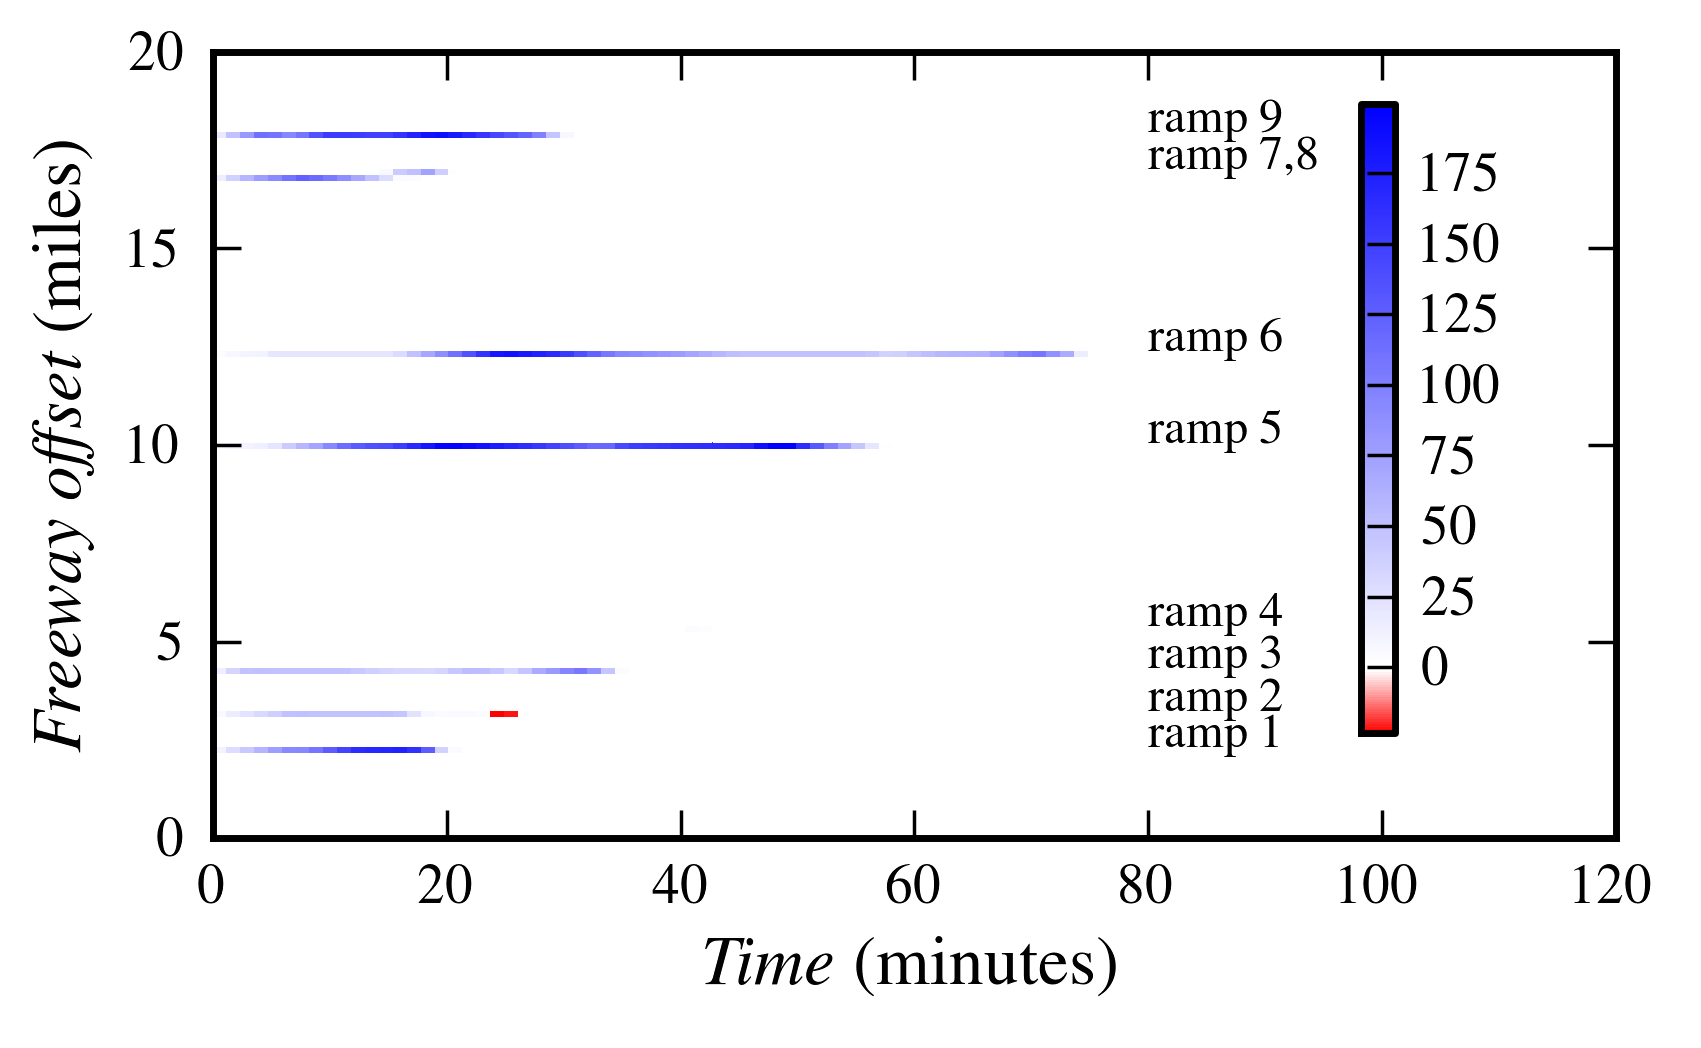
\includegraphics[width=0.45\columnwidth]{../images/queuediff}

}
\end{figure}

\end{frame}

\begin{frame}{Model predictive control}

\begin{itemize}
	\item Assume noisy state estimation and noisy predicted boundary flow data.
	\item About 2\% relative error in estimates.
	\item Every 15 minutes:
	\begin{itemize}
		\item Get state and boundary flow estimates over next 25 minutes.
		\item Produce policy for next 15 minutes.
	\end{itemize}
	\item Repeat for entire simulation horizon.
\end{itemize}
\end{frame}

\begin{frame}{Model predictive control}

\begin{figure}
\begin{centering}
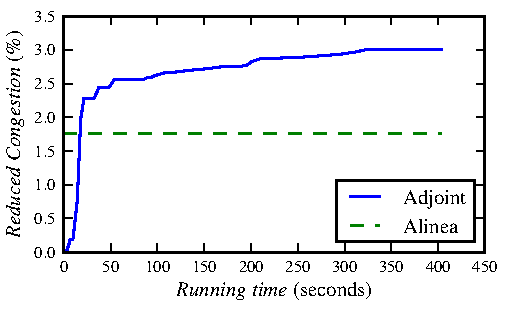
\includegraphics[width=0.8\columnwidth]{../images/longsim}
\par\end{centering}

\caption{Performance versus simulation time for freeway network. The results
indicate that the algorithm can run with performance better than Alinea
if given an update time around 15 minutes.}
\end{figure}

\end{frame}

\begin{frame}{Robustness to noise}

\begin{itemize}
	\item Adjoint method relies on reasonable input data estimates.
	\item If data is too noisy (>100\% relative error), reactive methods such as Alinea will outperform.
\end{itemize}

\begin{figure}
\subfloat[MPC performance on I15 South network.\label{fig:MPC-performance-on}]{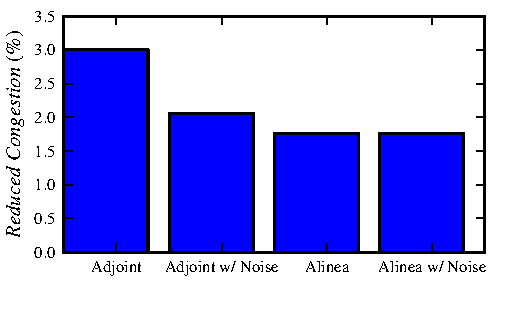
\includegraphics[width=0.45\columnwidth]{../images/longmpc}

}\hfill{}\subfloat[MPC performance with increasing sensor noise.\label{fig:Ramp-metering-performance-1}]{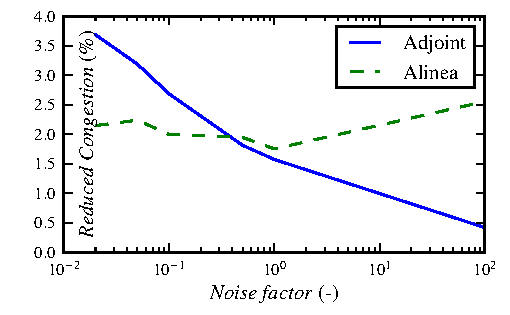
\includegraphics[width=0.45\columnwidth]{../images/noiseplot}

}
\end{figure}

\end{frame}

\begin{frame}{Partial control via rerouting}
...
\end{frame}


